\documentclass{article}
\usepackage{fullpage,amsmath,amsthm,graphicx,enumitem,amssymb}
\usepackage[hidelinks]{hyperref}
\usepackage{float}
\usepackage{tikz}
\usetikzlibrary{automata, positioning, arrows.meta, bending, decorations.pathmorphing}
\theoremstyle{definition}
\newtheorem{thm}{Theorem}
\newtheorem{question}[thm]{Question}
\newenvironment{solution}{\noindent\textit{Solution:}}{}
\usepackage{etoolbox}
\usepackage{bbm}

\newcommand{\reals}{\mathbb{R}}

\title{ASEN 5264 Decision Making under Uncertainty\\
       Homework 3: Online MDP Methods}

\begin{document}

\maketitle

A submission should consist of two or three files:
\begin{itemize}[nosep]
    \item A single PDF file containing answers to questions (typed, handwritten, or exported notebook).
    \item JSON file output from \texttt{HW3.evaluate}.
    \item A code listing \emph{if the code is not included in the PDF}.
\end{itemize}

\section{Conceptual Questions}

\begin{question}(10 pts)
    \begin{enumerate}[label=\alph*),nosep]
        \item Suppose that the optimal value function $U^*$ for an MDP with discrete state and action spaces is known. Write an equation in terms of ($S$, $A$, $T$, $R$, $\gamma$) for extracting the optimal policy $\pi^*$ from $U^*$.
        % \item Consider the following continuous-space MDP: $S = \mathbb{R}$, $A = \mathbb{R}$, $T(s'|s, a) = \mathcal{N}(s + a, 1)$, $R(s, a) = -s^2 - a^2$, $\gamma = 0.9$. Suppose that we have calculated the optimal value function for this MDP and found that $U^*(s) = -10s^2$. What is the optimal policy $\pi^*(s)$? Justify your answer.
        \item Suppose you have an MDP defined by 
            \begin{itemize}[label={},nosep]
                \item {\color{purple}$S = [0, \infty)$}, $\quad A = \{0, 0.1, 1\}$, $\quad \gamma = 1.0$
                \item $T(s'|s, a) = \mathcal{U}([s+a, s+a+1])$
                \item $R(s, a) = - \mathbbm{1}(s \leq 1) - a$
            \end{itemize}
            and a policy $\tilde{\pi}$ with $U^{\tilde{\pi}}(s) = -2\cdot\mathbbm{1}(s \leq 1)$. If the current state is 0.8, which action maximizes $Q^{\tilde{\pi}}(s, a)$? Justify your answer.
    \end{enumerate}
\end{question}


\begin{question} (10 pts) Do similar $Q$ values imply similar rewards?
    Consider the following claim:
    \begin{quote}
    % If a policy $\pi$ satisfies $|Q^*(s, \pi^*(s)) - Q^*(s, \pi(s))| \leq \beta$ for all $s \in S$ for some $\beta > 0$, then it immediately follows that $|R(s, \pi^*(s)) - R(s, \pi(s))| \leq \beta$ for any $s \in S$.
    {\color{purple}Let $\beta$ be a positive constant. If a policy $\pi$ satisfies $|Q^*(s, \pi^*(s)) - Q^*(s, \pi(s))| \leq \beta$ for all $s \in S$, then it immediately follows that $|R(s, \pi^*(s)) - R(s, \pi(s))| \leq \beta$ for any $s \in S$.}
    % If $|Q^*(s, \pi^*(s)) - Q^*(s, a)| \leq \beta$, then $|\mathcal{R}(s, \pi^*(s)) - \mathcal{R}(s, a)| \leq \beta$.
    \end{quote}
    It turns out that this claim is incorrect.\footnote{Even seasoned researchers can be tripped up by this - this claim was erroneously made in the proof for Lemma 5 of the Sparse Sampling paper by Kearns, Mansour, and Ng \url{https://www.cis.upenn.edu/~mkearns/papers/sparsesampling-journal.pdf}.} In this exercise, you will formulate a counterexample demonstrating that it is false. Consider the MDP below:
    \begin{figure}[H]
        \centering
        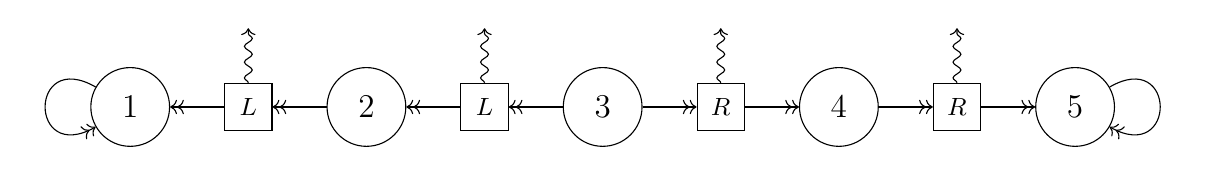
\begin{tikzpicture}[
            state/.style = {circle, draw, minimum size=1.0cm, font=\large},
            action/.style = {rectangle, draw, minimum size=0.6cm, font=\small},
            every edge/.style = {draw, thick},
        ]
            % States in a horizontal line
            \node[state] (1) at (0,0) {$1$};
            \node[state] (2) at (3,0) {$2$};
            \node[state] (3) at (6,0) {$3$};
            \node[state] (4) at (9,0) {$4$};
            \node[state] (5) at (12,0) {$5$};

            % Action nodes between states
            \node[action] (L1) at (1.5,0) {$L$};
            \node[action] (L2) at (4.5,0) {$L$};
            \node[action] (R3) at (7.5,0) {$R$};
            \node[action] (R4) at (10.5,0) {$R$};

            % Transitions: arrows point away from state 3
            % 3 -> L -> 2 -> L -> 1 (left side)
            \draw[->>] (3) -- (L2);
            \draw[->>] (L2) -- (2);
            \draw[->>] (2) -- (L1);
            \draw[->>] (L1) -- (1);
            % 3 -> R -> 4 -> R -> 5 (right side)
            \draw[->>] (3) -- (R3);
            \draw[->>] (R3) -- (4);
            \draw[->>] (4) -- (R4);
            \draw[->>] (R4) -- (5);

            % Absorbing state loops
            \draw[->>] (1) to[out=150, in=210, looseness=5] (1);
            \draw[->>] (5) to[out=30, in=-30, looseness=5] (5);

            % Reward arrows (squiggly) from action nodes
            \draw[->, decorate, decoration={snake, amplitude=0.5mm, segment length=2mm}] (L1) -- ++(0,1);
            \draw[->, decorate, decoration={snake, amplitude=0.5mm, segment length=2mm}] (L2) -- ++(0,1);
            \draw[->, decorate, decoration={snake, amplitude=0.5mm, segment length=2mm}] (R3) -- ++(0,1);
            \draw[->, decorate, decoration={snake, amplitude=0.5mm, segment length=2mm}] (R4) -- ++(0,1);
        \end{tikzpicture}
    \end{figure}
    The state space is $S = \{1, \ldots, 5\}$ and the action space is $A = \{L, R\}$ (but not all actions are available from each state). Transitions are deterministic as shown. The discount factor is $\gamma=0.9$.

    Choose a reward function, $R$, (i.e. values for the squiggly arrows), a policy, $\pi$, and a value $\beta$ that constitute a counterexample to the claim above.\footnote{To demonstrate that you have found a counterexample, use the following steps: (1) Choose $R$, $\pi$ and $\beta$ (note that to choose $\pi$, you only have to choose $\pi(3)$ because all other actions are pre-determined. (2) Verify that $Q^*(s, \pi^*(s))$ and $Q^*(s, \pi(s))$ are closer than $\beta$ for all states. (3) Find one state where the difference between $R(s, \pi^*(s))$ and $R(s, \pi(s))$ is greater then $\beta$. (4) If it is not possible, then revise $R$, $\pi$, and $\beta$ and try again.} Justify your answer.
\end{question}

\section{Exercises}
    \texttt{HW3.DenseGridWorld()} generates a 60x60 grid world MDP. There is a reward of +100 every 20 cells, i.e. at [20,20], [20,40], [40,20], etc. After the agent reaches one of these reward cells, the problem terminates. All cells also have a cost. Only a generative transition model is available. You will use the following functions from POMDPs.jl to interact with this problem (or larger versions) in the rest of this assignment:
    \begin{itemize}[nosep]
        \item \texttt{actions(m)}
        \item \texttt{@gen(:sp, :r)(m, s, a)}
        \item \texttt{isterminal(m, s)}
        \item \texttt{discount(m)}
        \item \texttt{statetype(m)}
        \item \texttt{actiontype(m)}
    \end{itemize}

\begin{samepage}
\begin{question} (15 pts) Monte Carlo Policy Evaluation
    \begin{enumerate}[label=\alph*)]
        \item Write a rollout simulation function for an MDP starting with the following code:
            \begin{verbatim}
        r_total = 0.0
        t = 0
        while !isterminal(mdp, s) && t < max_steps
            a = :down # replace this with a policy
            s, r = @gen(:sp,:r)(mdp, s, a)
            r_total += discount(m)^t*r
            t += 1
        end
                \end{verbatim} Use this function to perform a Monte Carlo evaluation of a uniform random policy on an MDP created with \texttt{HW3.DenseGridWorld(seed=3)}. Report the mean discounted reward estimate and standard error of the mean (SEM). Run enough simulations so that the SEM is less than 5.
         \item Create a heuristic policy that improves upon the random policy by at least 50 reward units. Report the mean and standard error from a Monte Carlo evaluation.
    \end{enumerate}
\end{question}
\end{samepage}

\begin{question} \label{q:mcts} (20 pts) Monte Carlo Tree Search
    
    Write code that performs 7 iterations of Monte Carlo Tree Search on an MDP created with \\
    \texttt{HW3.DenseGridWorld(seed=4)},
    starting at state $(19, 19)$. You will need to produce three dictionaries:
    \begin{itemize}[noitemsep]
        \item \texttt{Q} maps $(s, a)$ tuples to Q value estimates.
        \item \texttt{N} maps $(s, a)$ tuples to N, the number of times the node has been tried.
        \item \texttt{t} maps $(s, a, s')$ tuples to the number of times that transition was generated during construction of the tree.
    \end{itemize}
    Then visualize the resulting tree with \texttt{HW3.visualize\_tree(Q, N, t, SA[19, 19])}\footnote{\texttt{SA} is from the \texttt{StaticArrays.jl} package.}. \textbf{Submit an image of the tree, the code used to generate it, and a few sentences describing the tree after 7 iterations} (e.g. which actions have the highest Q values? Does this make sense?).
    
\end{question}

\begin{question}
    (15 pts) Planning with MCTS

    Use your Monte Carlo tree search from Question~\ref{q:mcts} to plan online in the simulation loop. Use 1000 iterations of MCTS to choose each action. Evaluate the MCTS planner with 100 100-step Monte Carlo simulations. Report the mean accumulated reward and standard error of the mean.
\end{question}

\section{Challenge Problem}

\begin{question}
    (10 pts code and description, 20 pts score) Fast Online Planning
    
    Create a function \texttt{select\_action(m,s)} that takes in a $100 \times 100$ \texttt{DenseGridWorld}, \texttt{m}, and a state \texttt{s}, and returns a near-optimal action. You may wish to base this code on the MCTS code that you wrote for Question~\ref{q:mcts}. Evaluate this function with \texttt{HW3.evaluate} and \textbf{submit the resulting \texttt{json} file along with the code and a one paragraph to one page description of your approach}, including tuning parameters that worked well, the rollout policy, etc. A score of 50 will receive full credit. In order to achieve a score above 50, you will be limited to 50ms of planning time per step. There are no restrictions on this problem - you may wish to use a different algorithm, multithreading, etc. Starter code on github will give suggestions for timing and other details.
\end{question}

\end{document}
